\documentclass[man,floatsintext]{apa6}
\usepackage{lmodern}
\usepackage{amssymb,amsmath}
\usepackage{ifxetex,ifluatex}
\usepackage{fixltx2e} % provides \textsubscript
\ifnum 0\ifxetex 1\fi\ifluatex 1\fi=0 % if pdftex
  \usepackage[T1]{fontenc}
  \usepackage[utf8]{inputenc}
\else % if luatex or xelatex
  \ifxetex
    \usepackage{mathspec}
  \else
    \usepackage{fontspec}
  \fi
  \defaultfontfeatures{Ligatures=TeX,Scale=MatchLowercase}
\fi
% use upquote if available, for straight quotes in verbatim environments
\IfFileExists{upquote.sty}{\usepackage{upquote}}{}
% use microtype if available
\IfFileExists{microtype.sty}{%
\usepackage{microtype}
\UseMicrotypeSet[protrusion]{basicmath} % disable protrusion for tt fonts
}{}
\usepackage{hyperref}
\hypersetup{unicode=true,
            pdftitle={Understanding the impacts of video-guided activities on parent-child interaction},
            pdfauthor={George Kachergis, Emily Hembacher, Veronica Cristiano, Hanwen Vivian Zhang, \& Michael C. Frank},
            pdfkeywords={digital parenting advice; joint attention; lexical diversity; guided play},
            pdfborder={0 0 0},
            breaklinks=true}
\urlstyle{same}  % don't use monospace font for urls
\usepackage{graphicx,grffile}
\makeatletter
\def\maxwidth{\ifdim\Gin@nat@width>\linewidth\linewidth\else\Gin@nat@width\fi}
\def\maxheight{\ifdim\Gin@nat@height>\textheight\textheight\else\Gin@nat@height\fi}
\makeatother
% Scale images if necessary, so that they will not overflow the page
% margins by default, and it is still possible to overwrite the defaults
% using explicit options in \includegraphics[width, height, ...]{}
\setkeys{Gin}{width=\maxwidth,height=\maxheight,keepaspectratio}
\IfFileExists{parskip.sty}{%
\usepackage{parskip}
}{% else
\setlength{\parindent}{0pt}
\setlength{\parskip}{6pt plus 2pt minus 1pt}
}
\setlength{\emergencystretch}{3em}  % prevent overfull lines
\providecommand{\tightlist}{%
  \setlength{\itemsep}{0pt}\setlength{\parskip}{0pt}}
\setcounter{secnumdepth}{0}
% Redefines (sub)paragraphs to behave more like sections
\ifx\paragraph\undefined\else
\let\oldparagraph\paragraph
\renewcommand{\paragraph}[1]{\oldparagraph{#1}\mbox{}}
\fi
\ifx\subparagraph\undefined\else
\let\oldsubparagraph\subparagraph
\renewcommand{\subparagraph}[1]{\oldsubparagraph{#1}\mbox{}}
\fi

%%% Use protect on footnotes to avoid problems with footnotes in titles
\let\rmarkdownfootnote\footnote%
\def\footnote{\protect\rmarkdownfootnote}


  \title{Understanding the impacts of video-guided activities on parent-child interaction}
    \author{George Kachergis\textsuperscript{1}, Emily Hembacher\textsuperscript{2}, Veronica Cristiano\textsuperscript{3}, Hanwen Vivian Zhang\textsuperscript{4}, \& Michael C. Frank\textsuperscript{1}}
    \date{}
  
\shorttitle{Impacts of videos on parent-child interaction}
\affiliation{
\vspace{0.5cm}
\textsuperscript{1} Department of Psychology, Stanford University\\\textsuperscript{2} Nextdoor, Inc.\\\textsuperscript{3} Gallaudet University\\\textsuperscript{4} Cornell University}
\keywords{digital parenting advice; joint attention; lexical diversity; guided play\newline\indent Word count: 4510}
\usepackage{csquotes}
\usepackage{upgreek}
\captionsetup{font=singlespacing,justification=justified}

\usepackage{longtable}
\usepackage{lscape}
\usepackage{multirow}
\usepackage{tabularx}
\usepackage[flushleft]{threeparttable}
\usepackage{threeparttablex}

\newenvironment{lltable}{\begin{landscape}\begin{center}\begin{ThreePartTable}}{\end{ThreePartTable}\end{center}\end{landscape}}

\makeatletter
\newcommand\LastLTentrywidth{1em}
\newlength\longtablewidth
\setlength{\longtablewidth}{1in}
\newcommand{\getlongtablewidth}{\begingroup \ifcsname LT@\roman{LT@tables}\endcsname \global\longtablewidth=0pt \renewcommand{\LT@entry}[2]{\global\advance\longtablewidth by ##2\relax\gdef\LastLTentrywidth{##2}}\@nameuse{LT@\roman{LT@tables}} \fi \endgroup}


\usepackage{lineno}

\linenumbers
\usepackage{float}

\authornote{

Correspondence concerning this article should be addressed to Michael C. Frank, Stanford, CA 94305 USA. E-mail: \href{mailto:mcfrank@stanford.edu}{\nolinkurl{mcfrank@stanford.edu}}}

\abstract{
Early parenting practices play an important role in shaping the future outcomes of young children (Hart \& Risley, 1995; Heckman, 2006).
In particular, high-quality early interactions and language input appear to facilitate language learning and result in higher levels of school performance.
The rise of phone- and tablet-based parenting applications (``apps'') holds the promise of delivering low-cost, positive interventions on parenting style to a wide variety of populations.
Of special interest are the parents of very young children, who are often difficult to reach in other ways. Yet little is known about the effects of communicating to parents through app-based interventions.
We showed parents a short video depicting an age-appropriate parent-child activity from a commercial parenting app, and found that the quality of parent-child interactions increases in some ways as a result of the intervention.
Specifically, after watching the activity video, parents spoke more and made more bids for joint attention with the child.


}

\begin{document}
\maketitle

\hypertarget{introduction}{%
\section{Introduction}\label{introduction}}

The quantity and quality of early language input has been found to be strongly associated with later language and academic outcomes (Cartmill et al., 2013; Hart \& Risley, 1995; Hirsh-Pasek et al., 2015; Marchman \& Fernald, 2008). Thus, because of the potential for large downstream effects (Heckman, 2006), there is tremendous interest in interventions that change children's language environment.
And because parents define a large portion of that environment, especially before the onset of formal schooling, parent behavior is a critical locus for such interventions.
Many effective parenting interventions require large resource investments and require many hours of in-person contact (Gertler et al., 2014; Schweinhart et al., 2004), making implementation at scale a daunting proposition.
For this reason, many researchers targeting early language are interested in delivering parenting interventions remotely -- through texts, apps, and videos delivered on digital devices.
But what do parents take away from these short messages about what to do with or how to talk with their children?

The content provided by digital parenting interventions runs the gamut from general parenting messages and facts from child development research to specific advice and suggested activities.
A growing body of evidence suggests that these digital interventions can be effective across a range of cultures, income levels, and children's ages (for a review, see Breitenstein, Gross, \& Christophersen, 2014).
For example, in contrast to a face-to-face parent training intervention, a tablet-based version saw significantly higher session completion rates (51\% attendance vs.~85\% module completion) and comparable or larger effect sizes on parents' and children's (aged 2 to 5 years) behavior (Breitenstein, Fogg, Ocampo, Acosta, \& Gross, 2016).
Often, however, the theory of change presupposed by such interventions is relatively vague.
Both within and outside the realm of academic interventions, messages to parents of young children often seek to provide knowledge about some aspect of development (e.g., early language), often in tandem with a suggestion regarding activities.
Such messages are assumed to inform parents' choice of behaviors, spurring them to engage in some target activity, which is assumed to be more stimulating than what parents would have done otherwise.

This theory of change is typically grounded in ideas about guided play and early language stimulation.
Child-directed speech varies not only in quantity (i.e., the number of total tokens), but also in quality in terms of the diversity of the tokens (Malvern, Richards, Chipere, \& Durán, 2004) or the context-appropriateness of the speech (Cartmill et al., 2013), both of which have been linked to children's subsequent language development.
Further, language learning -- especially the acquisition of early vocabulary in the first years -- appears to be supported preferentially by parents and children \emph{jointly attending} to some object or activity (Baldwin, 1991; Bigelow, MacLean, \& Proctor, 2004).
Episodes of joint attention are frequent during guided play, when parents set goals and scaffold their child's activities (Weisberg, Hirsh-Pasek, \& Golinkoff, 2013; Wood, Bruner, \& Ross, 1976).
Thus, the current literature supports interventions that encourage parents to provide high-quality language and interaction through something like guided play -- whether via reading books or playing with a shape-sorter at home, or via a conversation about categories in the supermarket.

But is this theory of change correct? That is, does the provision of knowledge and activities lead to higher-quality play?
Alternatively, by focusing parents on a specific activity, this theory could be flawed, causing parents to over-focus on achieving the superficial goals of the activity.
This problem might be especially likely with video messages, which could encourage parents to try to mimic a model's specific speech and/or actions.
Attempting to reproduce such surface details of a video-guided activity could in turn result in less high-quality talk, with less responsiveness to their child's play.
Another possibility is that these messages might produce the desired effect, but only for those parents who already have a general orientation towards children's early learning.

Our current experiments were designed to make a direct test of this question: How do parents change their interactions with young children on the basis of short video parenting messages?
In two experiments, we collected data from parent-child dyads in a local children's museum.
We showed parents in the experimental group a single short video modeling an interactive toy-based activity along with a scientific justification.
Parents in the control group received either no video (Experiment 1) or a video of a recent finding in developmental psychology (Experiment 2).
We then gave the toys from the video to all dyads and videotaped their interactions, coding for language quantity and quality as well as joint attention.

\hypertarget{experiment-1}{%
\section{Experiment 1}\label{experiment-1}}

In Experiment 1, we invited parents of 6- to 24-month-old infants visiting the Children's Discovery Museum in San Jose to complete video-guided activities from a commerical parenting app that delivers digital parenting advice in the form of short videos.
Parents were randomly assigned to the video condition or the control condition; parents in the \emph{activity video} condition watched a video from the app (matched to their child's age), and then performed the activity with their child using the props from the video.
Parents in the \emph{control} condition did not watch an activity video, but were given a set of the same age-appropriate props and asked to play with their infants as they normally would at home.

\hypertarget{method}{%
\subsection{Method}\label{method}}

\hypertarget{participants.}{%
\subsubsection{Participants.}\label{participants.}}

60 infants (F = 43, M = 17) aged 6-24 months (20 6-11.9 month-olds, 20 12-17.9 month-olds, and 20 18-24 month-olds) and their parents participated in a museum in northern California.
We included infants who were exposed to English at least 50 percent of the time (n = 58) or who were exposed less but whose participating parent reported that they primarily speak English with their child at home (n = 2).
62\% of participants (n = 37) had been exposed to two or more languages, as indicated by their parent.
Parents identified their children as White (n = 25), Asian (n = 11), African American/Black (n = 2), Biracial (n = 12), other (n = 5), or declined to state (n = 5).
Fifteen parents reported that their child was of Hispanic origin.
Parents tended to be highly-educated, with reports of highest level of education ranging from completed high school (n = 5), some college (n = 7), four-year college (n = 16), some graduate school (n = 2), to completed graduate school (n = 30).

\hypertarget{materials.}{%
\subsubsection{Materials.}\label{materials.}}

Stimuli included activity videos from a commercial parenting application.
The videos were designed to show activities to parents that they could perform with their child in order to foster cognitive and physical development, and were targeted to the child's age and level of development.
In each video, an adult and child perform the activity (e.g., sorting toys according to size) while a narrator explains the activity and its purpose.
We selected two videos for each of three age groups in our sample (6-11.9 months, 12-17.9 months, 18-23.94 months).
Participants were also given a set of toys corresponding to those in the video that they watched so that they could complete the activity.\footnote{Details of the specific videos used and the toys associated with each video are in the Appendix.}

Participants were randomly assigned to either the \emph{Activity Video} condition or the \emph{No Video} condition.
Parents participating in the Activity Video condition were assigned to watch one of the two activity videos available for their child's age group, while parents in the No Video condition watched no video, and were simply asked to play with their child as they normally would.
The No Video condition was yoked to the Activity Video condition such that for every participant in the Video condition who saw a particular video and received the associated props, a participant in the No Video condition received the same props but did not watch the activity video.
Parents also completed the Early Parenting Attitudes Questionnaire (EPAQ; Hembacher \& Frank, 2018).
The EPAQ measures parents of young children's attitudes about parenting and child development along three dimensions: rules and respect, early learning, and affection and attachment.

\hypertarget{procedure.}{%
\subsubsection{Procedure.}\label{procedure.}}

After providing informed consent, parents in the Activity Video condition watched the assigned activity video on a laptop with headphones.
To ensure that parents could give the video their full attention, the experimenter played with the infant with a set of toys (different from the experimental props used in the study) while the video was being played.
Immediately following the video, each parent-child dyad was provided with the props to complete the video-guided activity that the parent had viewed.
The toys were placed on a large foam play mat, and parents were instructed to sit on the mat with their child and re-create the activity they had viewed for a period of three minutes.\footnote{Based on piloting, we estimated these activities would would only require three minutes to complete.}
In the Control condition, after informed consent parents were told to play with their child as they would at home with the provided props for a period of three minutes.
They were not given any additional instructions about how to use the props.

In both conditions, two video cameras were used to record the play session from different angles, and parents were fitted with a wireless Shure lavalier microphone to record their child-directed speech.
After three minutes of play had elapsed, parents were told they could stop playing and the cameras and microphone were turned off.
Parents were then asked to complete the EPAQ before being debriefed.

\hypertarget{joint-attention-coding-procedure.}{%
\subsubsection{Joint Attention Coding Procedure.}\label{joint-attention-coding-procedure.}}

The video of each session was manually coded for episodes of joint attention (JA) using the Datavyu software (Team, 2014).
The video taken at floor level was coded by default, but the other video was referred to if the participants were occluded or if there was technical difficulty with the first camera.
Each session's video was coded for episodes of coordinated JA, episodes of passive JA, and parental bids for JA.
Parental bids for JA were defined as any attempt to initiate joint attention (i.e labeling, pointing, or otherwise drawing attention to an object) that did not result in passive or coordinated JA.
If more than 3 seconds elapsed between bids, they were coded as separate attempts.
An episode of joint attention was considered \emph{passive} if both participants visually focused on an object for 3 or more seconds but the child did not acknowledge the parent.
If either participant looked away from the object for less than 3 seconds and then returned to the same object it was considered part of the same episode of joint attention.
A joint attention episode was considered \emph{coordinated} if both participants visually focused on an object for 3 or more seconds and at some point in the interaction the child indicated awareness of interaction with some overt behavior toward the parent such as looking at their face, gesturing, vocalizing, or turn-taking.
Full details of our guidelines for coding joint attention are available in SI.

A second coder independently coded a third of the videos (i.e., 20 of the 60 videos, approximately equally distributed across ages) to establish reliability.
The two coders had a reliability of ICC = 0.80 with 95\% confident interval (CI) = {[}0.57,0.92{]} for number of parent bids for JA; ICC = 0.20 with 95\% CI = {[}-0.26,0.58{]} for number of passive JA episodes; ICC = 0.66 with 95\% CI = {[}0.32,0.85{]} for number of coordinated JA episodes; ICC = 0.24 with 95\% CI = {[}-0.21,0.61{]} for total duration of passive JA episodes, and ICC = 0.62 with 95\% CI = {[}0.27,0.83{]} for total duration of coordinated JA episodes.

\hypertarget{results}{%
\subsection{Results}\label{results}}

Parents' child-directed speech during the play sessions was transcribed.
The transcripts and hand-coded joint attention data were analyzed according to our preregistration\footnote{Preregistration: \url{https://osf.io/2bpdf/}{]}}, with any deviations or extensions noted.
Below we first report the lexical diversity results, followed by the joint attention results.

\hypertarget{lexical-diversity}{%
\subsubsection{Lexical Diversity}\label{lexical-diversity}}

For each transcript, the words were lemmatized using \texttt{spacy2} (Honnibal, 2017), and the word \emph{types} (unique words) and \emph{tokens} (total words) were then tallied and the type-token ratio (TTR) calculated as a measure of lexical diversity.
Although TTR was our preregistered measure of lexical diversity as it has commonly been used, it has been noted that TTR is correlated with the length of a text, which has led to the development of new measures such as the measure of textual lexical diversity (MTLD; McCarthy \& Jarvis, 2010).
Thus, we also measure lexical diversity with MTLD, which is calculated as the mean length of sequential word strings in a text that maintain a given TTR value (here we use the value proposed by McCarthy and Jarvis (2010): 0.720).

We fit a Bayesian mixed-effects linear regression predicting TTR as a function of condition, age (centered), gender, and parent's education level with a random intercept per video using rstanarm (Goodrich, Gabry, Ali, \& Brilleman, 2018).
For effects that are at least 95\% likely to be non-zero according to the posterior distribution, we report estimated coefficients (\(\beta\)) as well as 95\% Bayesian credible intervals (95\% CI), demarcating the range within which 95\% of the posterior predictive values fall.
There was significantly lower TTR in the Video condition (mean: 0.32) than in the Control condition (mean: 0.43, \(\beta=\)-0.11, 95\% CI={[}-0.16,-0.06{]}).
There were no significant effects of age, gender, or parent's level of education.
A similar Bayesian mixed-effects linear regression instead predicting MTLD also found significantly lower lexical diversity in the Video condition (mean MTLD: 17.87) than in the Control condition (mean: 27.09, \(\beta=\)-8.62, 95\% CI={[}-15.15,-2.01{]}), with no other significant effects.
Figure \ref{fig:lexdiv} shows the mean of each lexical diversity measure (TTR and MTLD) by condition.

We also conducted similar regressions predicting the number of word tokens and types, finding only a significant effect of condition on the number of word tokens (\(\beta=\) 56.36, 95\% CI={[}14.02,96.32{]})), with parents using more words in the Video condition (mean: 225, bootstrapped 95\% confidence intervals (CI): {[}199,252{]}) than in the Control condition (mean: 165, bootstrapped 95\% CI: {[}139,193{]}).

\begin{figure}[H]

{\centering 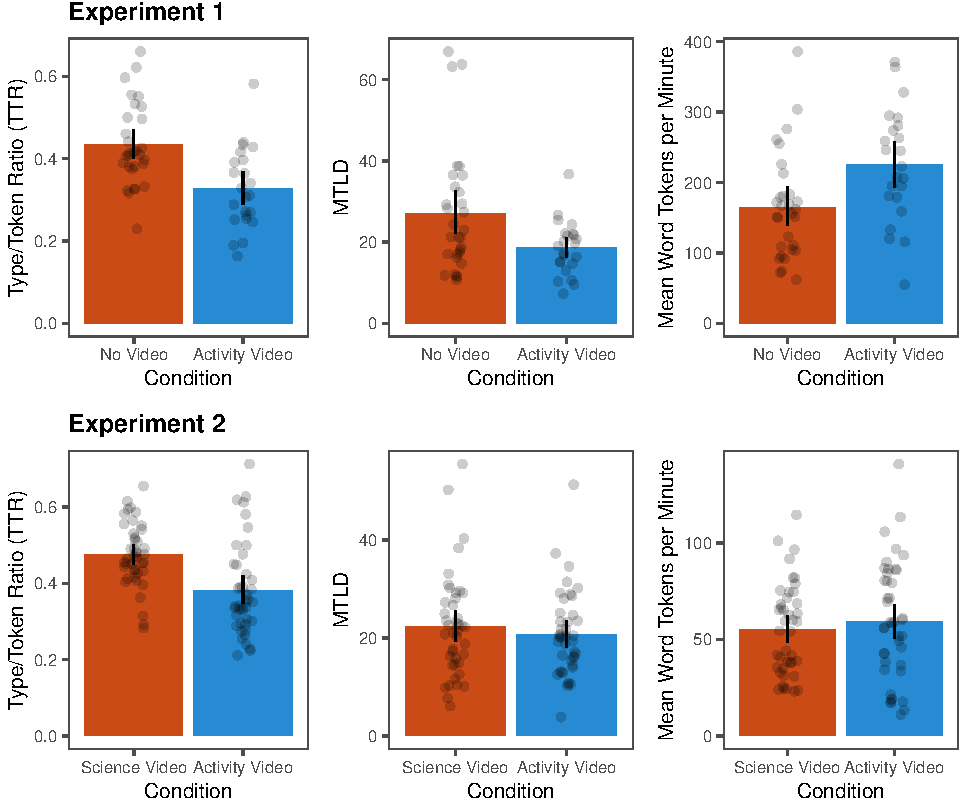
\includegraphics{figs/fig-lexdiv-1} 

}

\caption{\label{fig:lexdiv} Mean lexical diversity scores (left: Type/Token ratio, middle: MTLD) and mean number of tokens used by condition (right) in Experiment 1 (top) and Experiment 2 (bottom). Error bars show bootstrapped 95\% confidence intervals (CIs), and gray dots indicate values for each participant.}\label{fig:fig-lexdiv}
\end{figure}

\hypertarget{joint-attention}{%
\subsubsection{Joint Attention}\label{joint-attention}}

We fit a mixed-effects linear regression predicting the number of bids for joint attention (JA) as a function of fixed effects of condition, age (centered), gender, parent's education level, and the subscales of the EPAQ: Early Learning (EL), Affection and Attachment (AA), and Rules and Respect (RR), along with interactions of condition and EL, AA, and RR.
This model included random intercepts per video.
There were significantly more bids for JA in the Video condition (mean: 6.30, sd: 2.76) than in the Control condition (mean: 3.73, sd: 2.74, \(\beta=3.40\), 95\% CI={[}1.03,5.73{]}).

Mixed-effects regressions with the same structure were performed predicting the number of episodes of coordinated and passive JA, and the total duration of time spent in coordinated and passive JA.
There were no significant effects on the number or total duration of coordinated JA episodes, nor on the total duration of passive JA episodes.
For the regression predicting the number of passive JA episodes, the only significant effect was an interaction of condition and RR (\(\beta=1.82\), 95\% CI={[}0.20,3.48{]}), showing that for parents in the Video condition, those with higher Rules and Respect subscores engaged in more passive JA episodes.
Figure \ref{fig:JA} (top) shows the mean number bids for JA and episodes of JA by condition in Experiment 1.

\begin{figure}[H]

{\centering 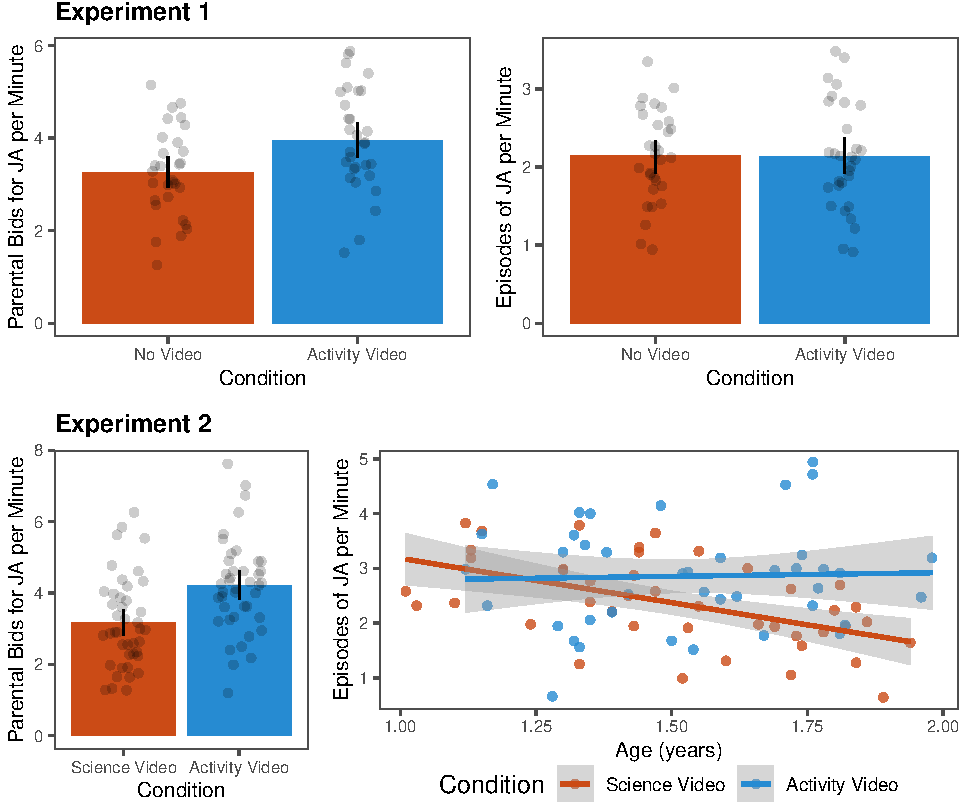
\includegraphics{figs/fig-JA-1} 

}

\caption{\label{fig:JA} Mean number of bids (left) and episodes (right) of joint attention (JA) by condition in Experiment 1 (top). For Experiment 2 (bottom), mean number of bids for JA by condition (left) and the number of episodes of JA by age and condition (right).}\label{fig:fig-JA}
\end{figure}

\hypertarget{discussion}{%
\subsection{Discussion}\label{discussion}}

In summary, while parents produced more word types and tokens after viewing the activity video, lexical diversity (both TTR and MTLD) was higher when parents were just asked to play as they normally would.
It may be that parents in the Activity Video condition, in their attempt to stick to the prescribed task, end up repeating themselves more.
Looking at the most frequent content words parents used after the Activity Video, \ldots{}
In contrast, the most frequent content words parents used in the Control condition were\ldots{}

Parents who watched an activity video made significantly more bids for JA with their child, although this did not result in a greater number of successful episodes of JA than dyads in the no video condition.
No differences in the duration or number of episodes of passive or coordinated JA between conditions were found.

After the activity video, parents with higher RR scores showed an increased number of passive JA episodes than high-RR parents did after no video.
While the electronically-delivered parenting advice increased the number of bids for JA by parents, it did not significantly affect the number or duration of episodes of JA.
RELATE BACK TO HYPOTHESES

\hypertarget{experiment-2}{%
\section{Experiment 2}\label{experiment-2}}

Experiment 1 found that parents who watched an activity video spoke more words overall, but had lower lexical diversity compared to parents who played with their children as they normally would at home.
Might it be that parents who are focused on a specific activity show reduced lexical diversity due to their focus on engaging their child in the activity?
Parents who watched an activity video made more bids for joint attention, although these bids did not result in more episodes of joint attention compared to the control group.
Experiment 2 attempts to replicate these findings from with a restricted number of preregistered predictions.\footnote{Preregistration: \url{https://osf.io/2bpdf/}.}

\hypertarget{method-1}{%
\subsection{Method}\label{method-1}}

\hypertarget{participants.-1}{%
\subsubsection{Participants.}\label{participants.-1}}

84 infants (F = 36, M = 46) aged 12-24 months (41 12-17.9 month-olds, 43 18-24 month-olds) and their parents participated in the same museum as Experiment 1.
We included infants who were exposed to English at least 75 percent of the time or who were exposed less but whose participating parent reported that they primarily speak English with their child at home.
Forty-nine percent of participants (n = 41) had been exposed to two or more languages as indicated by their parent.
Parents identified their children as White (n = 39), Asian (n = 20), African American/Black (n = 1), Biracial (n = 9), other (n = 7), or declined to state (n = 8).
Sixteen parents reported their child was of Hispanic origin.
Parents tended to be highly-educated, with reports of highest level of education ranging from some college (n = 5), four-year college (n = 28), some graduate school (n = 2), to completed graduate school (n = 36) or declined to state (n = 13).

\hypertarget{materials.-1}{%
\subsubsection{Materials.}\label{materials.-1}}

The design of Experiment 2 was similar to that of Experiment 1, except that instead of No Video control condition, parents instead watched a video that was generally related to child development research, but did not give any specific instructions about how to interact with infants or children.
This condition was included to control for the possibility that differences in language output and joint attention in Experiment 1 could be due to simply cueing parents to think about infants' learning and cognitive development.
The videos presented in the Control Video condition were media clips (available on YouTube) of developmental psychologists explaining their research interleaved with footage of infants or toddlers engaged in developmental research studies.
Thus, the content of the videos superficially matched those in the Activity Video condition, but did not suggest any particular activities.
The videos were trimmed to approximately match the average video length in the Activity Video condition (close to 90 s).
Details of the videos used in the Activity Video conditions are in the Appendix.

\hypertarget{procedure.-1}{%
\subsubsection{Procedure.}\label{procedure.-1}}

The procedure for Experiment 2 matched that of Experiment 1, except that parents in the Control Video condition watched a control video before the play session.
Consistent with the No-Video control condition in Experiment 1, parents in the Control Video condition were told to play with their child as they would at home, and were not given additional instructions.
The coding procedure also matched that of Experiment 1.
A second coder independently coded a third of the videos (i.e., 26 of the 84 videos, approximately equally distributed across ages) to establish reliability.
The two coders had a reliability of ICC = 0.80 with 95\% confidence interval (CI) = {[}0.60,0.90{]} for number of parent bids for JA; ICC = 0.74 with 95\% CI = {[}0.59,0.87{]} for number of passive JA episodes; ICC = 0.78 with 95\% CI = {[}0.58,0.90{]} for number of coordinated JA episodes; ICC = 0.72 with 95\% CI = {[}0.46,0.86{]} for total duration of passive JA episodes, and ICC = 0.88 with 95\% CI = {[}0.75,0.94{]} for total duration of coordinated JA episodes.

\hypertarget{results-1}{%
\subsection{Results}\label{results-1}}

Parents' child-directed speech was transcribed and processed, and bids and episodes of joint attention were coded according to the same procedure used in Experiment 1.
We first report reregistered regressions predicting TTR and number of tokens, as well as an exploratory regression predicting MTLD.
We then turn to preregistered regressions of parental bids for joint attention and the total number of JA episodes.
As noted in the preregistration, we adopt an alpha level of .005 for statistical significance and will report alphas between .05 and .005 as suggestive.

\hypertarget{lexical-diversity-1}{%
\subsubsection{Lexical Diversity}\label{lexical-diversity-1}}

We fit a mixed-effects linear regression predicting TTR as a function of age (centered) and condition with an interaction term, and with random intercepts per video using lme4 (Bates, Mächler, Bolker, \& Walker, 2015).
There was suggestively lower TTR in the Video condition (mean: 0.38) than in the Control condition (mean: 0.48, \(\beta=-0.09\), , 95\% CI={[}-0.15,-0.03{]}).
There was no significant effect of age, nor a significant interaction.
The preregistered regression predicting the number of tokens used by parents revealed no significant effects.
An exploratory mixed-effects linear regression predicting MTLD found no significant effects of age or condition.
Figure \ref{fig:lexdiv} (bottom left and middle) shows the mean of each lexical diversity measure (TTR and MTLD) by condition.
Regressions with the same structure predicting the number of words tokens found no significant effects of age or condition.
The means of the lexical measures are shown in Table \ref{e2tab}.

\begin{table}[t]

\caption{\label{tab:e2tab}\label{e2tab} Lexical diversity measures in Experiment 2.}
\centering
\begin{tabular}{l|r|r|r|r|r|r|r|r}
\hline
Condition & TTR (M) & (sd) & MTLD (M) & (sd) & Types (M) & (sd) & Tokens (M) & (sd)\\
\hline
Science Video & 0.48 & 0.08 & 22.45 & 10.57 & 86.83 & 26.87 & 191.38 & 72.08\\
\hline
Activity Video & 0.38 & 0.12 & 20.63 & 8.66 & 80.95 & 24.14 & 234.60 & 92.68\\
\hline
\end{tabular}
\end{table}

\hypertarget{joint-attention-1}{%
\subsubsection{Joint Attention}\label{joint-attention-1}}

As preregistered, we fit mixed-effects linear regressions predicting the number of parental bids for joint attention and the total number of episodes of JA as a function of fixed effects of condition, age (centered), and their interaction, with random intercepts per video.
Shown in Figure \ref{fig:JA} (left bottom), parents made significantly more bids for JA after watching the Activity Video (mean: 12.96, bootstrapped 95\% CI: 11.79, 14.24; \(\beta=3.07\), 95\% CI = {[}1.15,5.06{]}) than after the Science Video (mean: 9.89, 95\% CI: {[}8.73, 11.10{]}).
There were no other significant effects on parental bids for JA.

In the regression predicting the number of episodes of JA, there was a significant main effect of condition (\(\beta=1.48\), 95\% CI = {[}0.15,2.78{]}), with more episodes of JA occurring after the Activity Video (mean: 8.80, 95\% CI: {[}7.97, 9.63{]}) than after the Control Video (mean: 7.33, 95\% CI: {[}6.58, 8.11{]}).
There was also a significant main effect of age (\(\beta=-5\), 95\% CI = {[}-8.27,-1.41{]}), showing that the number of episodes of JA decreased with the child's age.
However, a significant interaction of age and condition (\(\beta=5.60\), 95\% CI = {[}0.46,10.37{]}), shown in Figure \ref{fig:JA} (right bottom), demonstrates that older children in the Activity Video condition did not see a decrease in the number of episodes of JA.

\hypertarget{exploratory-analyses}{%
\subsubsection{Exploratory Analyses}\label{exploratory-analyses}}

Four additional exploratory regressions with a similar structure were carried out to predict the number and duration of coordinated and passive JA episodes.
The regression predicting the number of episodes of coordinated JA found a significant main effect of condition (\(\beta=1.35\), 95\% CI = {[}0.17,2.61{]}), with more episodes of coordinated JA occurring after the Activity Video (mean: 6.72, 95\% CI: {[}5.91, 7.56{]}) than after the Control Video (mean: 5.33, 95\% CI: {[}4.70, 5.97{]}).
There was no significant effect of age, but there was a significant interaction of age and condition (\(\beta=5.28\), 95\% CI = {[}0.52,10.02{]}), shown in Figure \ref{fig:e2ja-coord}, revealing that older children in the Activity Video condition had more episodes of coordinated JA than children in the Control Video condition.
The regression predicting the total duration of coordinated JA episodes revealed no significant effects.

In the regression predicting the number of episodes of passive JA, there was a main effect of age (\(\beta=-2.70\), 95\% CI = {[}-5.07,0.08{]}), showing that older children had more episodes of passive JA with their caregiver.
The regression predicting the total duration of passive JA revealed a main effect of age (\(\beta=-18.32\), 95\% CI = {[}-33.50,-2.91{]}), revealing that older children spent more time in passive JA with their caregiver.
Overall, these results show that the older children in our sample engage in more and longer episodes of joint attention with their caregivers, and suggest that the Activity Video strengthened this trend in the number of episodes of coordinated JA.

\begin{figure}[H]

{\centering 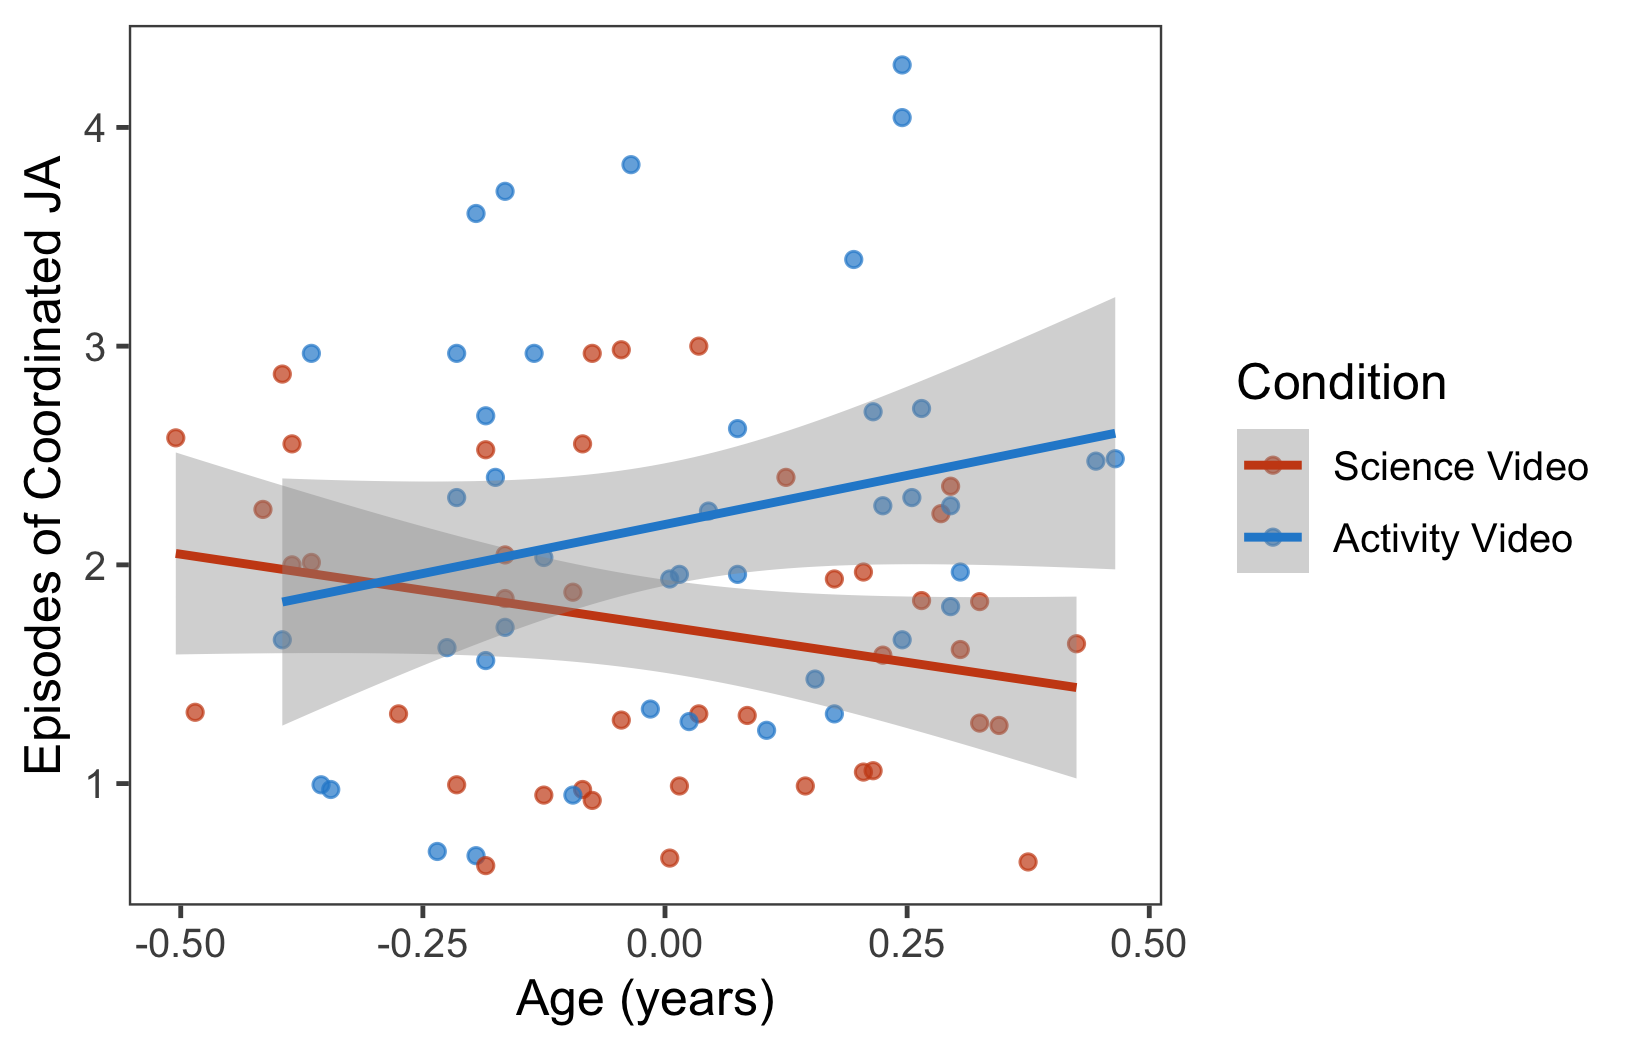
\includegraphics{figs/e2ja-coord-1} 

}

\caption{The number of episodes of coordinated JA by condition and age in Experiment 2. Older children in the Activity Video condition engaged in more episodes of coordinated JA with their caregiver than dyads in the Control Video condition.}\label{fig:e2ja-coord}
\end{figure}

\hypertarget{discussion-1}{%
\section{Discussion}\label{discussion-1}}

This study investigated how parents change their interactions with their young children on the basis of one of several short video parenting messages from a commercial parenting app, which suggest interactive toy-based activities (e.g., learning animal sounds), along with a scientific justification.
Parents in the control conditions received either no video (Experiment 1) or a video of a recent finding in developmental psychology (Experiment 2), but played with the same sets of toys given to those in the experimental conditions.
After completing the videos, parents were videotaped playing with their children for two minutes.
The quality of parents' interactions with their children were measured by the lexical diversity of their child-directed speech, and through behavioral coding of bids for and episodes of joint attention (JA).

Experiment 1 investigated 6--24-month-olds, and found a greater number of bids for JA from parents after watching the activity video, but no difference in the number of JA episodes.
Experiment 2 (12--24-month-olds) replicated this greater number of bids for JA after the activity video, and moreover found that while the number of JA episodes dwindled for older infants in the control condition, dyads in the activity video condition achieved an overall higher and constant number of JA episodes.
In combination, these results suggest that short parenting messages suggesting activities can encourage parents to make more attempts to engage their child in joint attention, and that in some cases--especially in older children--these bids are successful in increasing engagement.

Experiment 1 found lower lexical diversity in parents' speech after watching the activity video, but the average number of word tokens used was higher after the activity video, and the number of word types was the same in both conditions.
Experiment 2 had similar lexical diversity results, finding suggestively lower Type-Token Ratio after the activity video, although the length-corrected lexical diversity measure (MTLD) did not differ significantly.
However, neither the number of tokens nor the number of types significantly differed betwen conditions in Experiment 2.
Although it may at first blush seem worrisome that the activity videos lead to somewhat lower lexical diversity, this worry is mitigated by the fact that this difference is explained not by fewer word types but by a greater number of word tokens used by parents after the activity video (significantly in Experiment 1, and numerically in Experiment 2).
It may be that parents are relatively more repetitive after watching the activity video in their attempt to stick to the prescribed task, but overall they talk more.

Taken together, the results of this study show that digital parenting interventions recommending particular play activities to parents of young children can influence both the quality and quantity of child-directed speech, as well as parents attempts to engage their children in joint attention---at least in the short term.
Future studies should investigate whether these changes in parents' speech and attempts to engage their children continue after the treatment.
Another target for future study is to determine whether, over a longer treatment period, children begin to respond to the increased bids for joint attention and greater number of tokens by engaging more with their parent, and perhaps even beginning to play differently.

\hypertarget{acknowledgements}{%
\section{Acknowledgements}\label{acknowledgements}}

This work was supported by a gift from Kinedu, Inc.
Thanks to members of the Language and Cognition Lab at Stanford for helpful discussion.

\newpage

\hypertarget{references}{%
\section{References}\label{references}}

\begingroup
\setlength{\parindent}{-0.5in}
\setlength{\leftskip}{0.5in}

\hypertarget{refs}{}
\leavevmode\hypertarget{ref-Baldwin1991}{}%
Baldwin, D. (1991). Infants' contribution to the achievement of joint reference. \emph{Child Development}, \emph{62}, 875--890.

\leavevmode\hypertarget{ref-lme4}{}%
Bates, D., Mächler, M., Bolker, B., \& Walker, S. (2015). Fitting linear mixed-effects models using lme4. \emph{Journal of Statistical Software}, \emph{67}(1), 1--48. \url{http://doi.org/10.18637/jss.v067.i01}

\leavevmode\hypertarget{ref-Bigelow2004}{}%
Bigelow, A. E., MacLean, K., \& Proctor, J. (2004). The role of joint attention in the development of infants' play with objects. \emph{Developmental Science}, \emph{7}, 518--526.

\leavevmode\hypertarget{ref-Breitenstein2016}{}%
Breitenstein, S. M., Fogg, L., Ocampo, E. V., Acosta, D. I., \& Gross, D. (2016). Parent use and efficacy of a self-administered, tablet-based parent training intervention: A randomized controlled trial. \emph{JMIR mHealth and uHealth}, \emph{4}(2), e36. \url{http://doi.org/10.2196/mhealth.5202}

\leavevmode\hypertarget{ref-Breitenstein2014}{}%
Breitenstein, S. M., Gross, D., \& Christophersen, R. (2014). Digital delivery methods of parenting training interventions: A systematic review. \emph{Worldviews on Evidence-Based Nursing}, \emph{11}, 168--176.

\leavevmode\hypertarget{ref-Cartmill2013}{}%
Cartmill, E. A., Armstrong, B. F., Gleitman, L. R., Goldin-Meadow, S., Medina, T. N., \& Trueswell, J. C. (2013). Quality of early parent input predicts child vocabulary 3 years later. \emph{Proceedings of the National Academy of Sciences}, \emph{110}(28), 11278--11283. \url{http://doi.org/10.1073/pnas.1309518110}

\leavevmode\hypertarget{ref-Jamaica2014}{}%
Gertler, P., Heckman, J., Pinto, R., Zanolini, A., Vermeersch, C., Walker, S., \ldots{} Grantham-McGregor, S. (2014). Labor market returns to an early childhood stimulation intervention in jamaica. \emph{Science}, \emph{344}(6187), 998--1001. \url{http://doi.org/10.1126/science.1251178}

\leavevmode\hypertarget{ref-rstanarm}{}%
Goodrich, B., Gabry, J., Ali, I., \& Brilleman, S. (2018). Rstanarm: Bayesian applied regression modeling via Stan. Retrieved from \url{http://mc-stan.org/}

\leavevmode\hypertarget{ref-Hart1995}{}%
Hart, B., \& Risley, T. R. (1995). \emph{Meaningful differences in the everyday experience of young american children}. Baltimore, MD: Brookes.

\leavevmode\hypertarget{ref-Heckman2006}{}%
Heckman, J. J. (2006). Skill formation and the economics of investing in disadvantaged children. \emph{Science}, \emph{312}(5782), 1900--1902. \url{http://doi.org/10.1126/science.1128898}

\leavevmode\hypertarget{ref-Hembacher2018}{}%
Hembacher, E., \& Frank, M. C. (2018). The early parenting attitudes questionnaire: Measuring intuitive theories of parenting and child development. \emph{PsyArXiv}. \url{http://doi.org/10.31234/osf.io/hxk3d}

\leavevmode\hypertarget{ref-HirshPasek2015}{}%
Hirsh-Pasek, K., Adamson, L. B., Bakeman, R., Owen, M. T., Golinkoff, R. M., Pace, A., \ldots{} Suma, K. (2015). The contribution of early communication quality to low-income children's language success. \emph{Psychological Science}, \emph{26}(7), 1071--1083. \url{http://doi.org/10.1177/0956797615581493}

\leavevmode\hypertarget{ref-spacy2}{}%
Honnibal, I., Matthew AND Montani. (2017). SpaCy 2: Natural language understanding with bloom embeddings, convolutional neural networks and incremental parsing. \emph{To Appear}.

\leavevmode\hypertarget{ref-Malvern2004}{}%
Malvern, D., Richards, B. J., Chipere, N., \& Durán, P. (2004). \emph{Lexical diversity and language development}. Palgrave Macmillan.

\leavevmode\hypertarget{ref-Marchman2008}{}%
Marchman, V. A., \& Fernald, A. (2008). Speed of word recognition and vocabulary knowledge in infancy predict cognitive and language outcomes in later childhood. \emph{Developmental Science}, \emph{11}, F9--F16.

\leavevmode\hypertarget{ref-McCarthy2010}{}%
McCarthy, P. M., \& Jarvis, S. (2010). MTLD, vocd-d, and hd-d: A validation study of sophisticated approaches to lexical diversity assessment. \emph{Behavior Research Methods}, \emph{42}(2), 381--392.

\leavevmode\hypertarget{ref-PerryPreschool2004}{}%
Schweinhart, L. J., Montie, J., Xiang, Z., Barnett, W. S., Belfield, C. R., \& Nores, M. (2004). \emph{Lifetime effects: The highscope perry preschool study through age 40}. Ypsilanti, MI: HighScope Press.

\leavevmode\hypertarget{ref-datavyu}{}%
Team, D. (2014). Datavyu: A video coding tool. \emph{Databrary Project}. Retrieved from \url{http://datavyu.org}

\leavevmode\hypertarget{ref-Weisberg2013}{}%
Weisberg, D. S., Hirsh-Pasek, K., \& Golinkoff, R. M. (2013). Guided play: Where curricular goals meet a playful pedagogy. \emph{Mind, Brain, and Education}, \emph{7}, 104--112.

\leavevmode\hypertarget{ref-Wood1976}{}%
Wood, D., Bruner, J. S., \& Ross, G. (1976). The role of tutoring in problem solving. \emph{Journal of Child Psychology and Psychiatry}, \emph{17}, 89--100.

\endgroup

\clearpage
\makeatletter
\efloat@restorefloats
\makeatother


\begin{appendix}
\section{}
\hypertarget{experiment-1-activities}{%
\subsection{Experiment 1 Activities}\label{experiment-1-activities}}

\hypertarget{video-a-6-11.9-months-pick-it-up}{%
\subsubsection{Video A (6-11.9 months) ``Pick it
up''}\label{video-a-6-11.9-months-pick-it-up}}

Parents are told to encourage their child to pick up and drop individual
objects. They are also encouraged to place toys on a small cloth and
show the child that they can drag the cloth towards them to reach the
toys.

Props: cloth, plastic horse, plastic sheep, plastic elephant, toy car

\hypertarget{video-b-6-11.9-months-animal-sounds}{%
\subsubsection{Video B (6-11.9 months) ``Animal
sounds''}\label{video-b-6-11.9-months-animal-sounds}}

Parents are told to call different animals and imitate different sounds
the animals make. They are also encourgaed to observe which animal the
child prefers.

Props: plastic sheep, plastic horse, plastic frog, plastic cow, bowls

\hypertarget{video-c-12-17.9-months-give-me-the-toy}{%
\subsubsection{Video C (12-17.9 months) ``Give me the
toy''}\label{video-c-12-17.9-months-give-me-the-toy}}

Parents are told to ask their child to hand over individual toys. They
are also encouraged to praise the child after they give them the toys,
and repeat the process until the child could follow the verbal
instructions.

Props: toy boat, plastic frog, plastic elephant, toy bus

\hypertarget{video-d-12-17.9-months-classifying-my-toys}{%
\subsubsection{Video D (12-17.9 months) ``Classifying my
toys''}\label{video-d-12-17.9-months-classifying-my-toys}}

Parents are told to place toys of different sizes (big or small) in two
hoops. They are also encouraged to ask their child to distinguish
between two objects and identify which one is larger.

Props: two yellow and green rings, big car, small car, big horse, small
horse

\hypertarget{video-e-18-23.9-months-my-toys}{%
\subsubsection{Video E (18-23.9 months) ``My
toys''}\label{video-e-18-23.9-months-my-toys}}

Parents are told to show the child toys of the same shape but different
sizes, to place one of the objects in a basket and to ask the child to
take out the object. They are also encouraged to ask their child if the
object is bigger or smaller compared to its pair.

Props: two buckets, big car, small car, big horse, small horse

\hypertarget{video-f-18-23.9-months-the-orchestra}{%
\subsubsection{Video F (18-23.9 months) ``The
Orchestra''}\label{video-f-18-23.9-months-the-orchestra}}

Parents are told to give their child a musical instrument to play. They
are also encouraged to play a song and see if the child follows the
rhythm.

Props: maracas, drum, tambourine, clapper

\hypertarget{experiment-2-activities}{%
\subsection{Experiment 2 Activities}\label{experiment-2-activities}}

\hypertarget{video-a-12-17.9-months-give-me-the-toy}{%
\subsubsection{Video A (12-17.9 months) ``Give me the
toy''}\label{video-a-12-17.9-months-give-me-the-toy}}

Parents are told to ask their child to hand over individual toys. They
are also encouraged to praise the child after they give them the toys,
and repeat the process until the child could follow the verbal
instructions.

Props: plastic pig, plastic horse, plastic dog, plastic cat, plastic cow

\hypertarget{video-b-12-17.9-months-classifying-my-toys}{%
\subsubsection{Video B (12-17.9 months) ``Classifying my
toys''}\label{video-b-12-17.9-months-classifying-my-toys}}

Parents are told to place toys of different sizes (big or small) in two
hoops. They are also encouraged to ask their child to distinguish
between two objects and identify which one is larger.

Props: two yellow and green rings, big car, small car, big horse, small
horse

\hypertarget{video-c-12-17.9-months-geometric-shapes-jigzsaw-puzzle}{%
\subsubsection{Video C (12-17.9 months) ``Geometric shapes jigzsaw
puzzle''}\label{video-c-12-17.9-months-geometric-shapes-jigzsaw-puzzle}}

Parents are told to encourage their child to name different shapes on a
jigzsaw puzzle. Then they are told to undo the puzzle and invite the
child to complete the puzzle.

Props: A jigzsaw puzzle of geometric shapes

\hypertarget{video-d-18-23.9-months-my-toys}{%
\subsubsection{Video D (18-23.9 months) ``My
toys''}\label{video-d-18-23.9-months-my-toys}}

Parents are told to show the child toys of the same shape but different
sizes, to place one of the objects in a basket and to ask the child to
take out the object. They are also encouraged to ask their child if the
object is bigger or smaller compared to its pair.

Props: two buckets, big car, small car, big horse, small horse

\hypertarget{video-e-18-23.9-months-the-orchestra}{%
\subsubsection{Video E (18-23.9 months) ``The
Orchestra''}\label{video-e-18-23.9-months-the-orchestra}}

Parents are told to give their child a musical instrument to play. They
are also encouraged to play a song and see if the child follows the
rhythm.

Props: maracas, drum, tambourine, clapper

\hypertarget{video-f-18-23.9-months-my-yellow-toys}{%
\subsubsection{Video F (18-23.9 months) ``My Yellow
Toys''}\label{video-f-18-23.9-months-my-yellow-toys}}

Parents are told to show their child yellow toys and to ask, ``What
color are they?'' They are also told to give the child toys of different
colors, to ask them to only play with the yellow ones, and to praise the
child after they do so.

Props: blue car, yellow car, yellow block, red block, blue block, green
block
\end{appendix}


\end{document}
